\part{Qsim web}
\label{qsimweb}
La entrega de este trabajo cuenta con una librería que implementa la especificación de la arquitectura Q y una interfaz de usuario que permite hacer uso de la librería de una manera más didáctica.

La construcción de la librería fue realizada utilizando javascript. El parser utiliza la librería nearley. El testing unitario y de integración fue realizado con mocha y cypress.
La construcción de la interfaz de usuario fue realizada en React con la librería Material-UI y react-ace para el editor. 
Esta implementación esta subida a un servidor utilizando Heroku, en el siguiente link: \href{https://qweb-unq.herokuapp.com/}{https://qweb-unq.herokuapp.com/}.
Su código fuente está subido a Gitlab y puede verse en el siguiente link: \href{https://gitlab.com/qsim-web-project/qsim-web}{https://gitlab.com/qsim-web-project/qsim-web}.
\begin{center}
  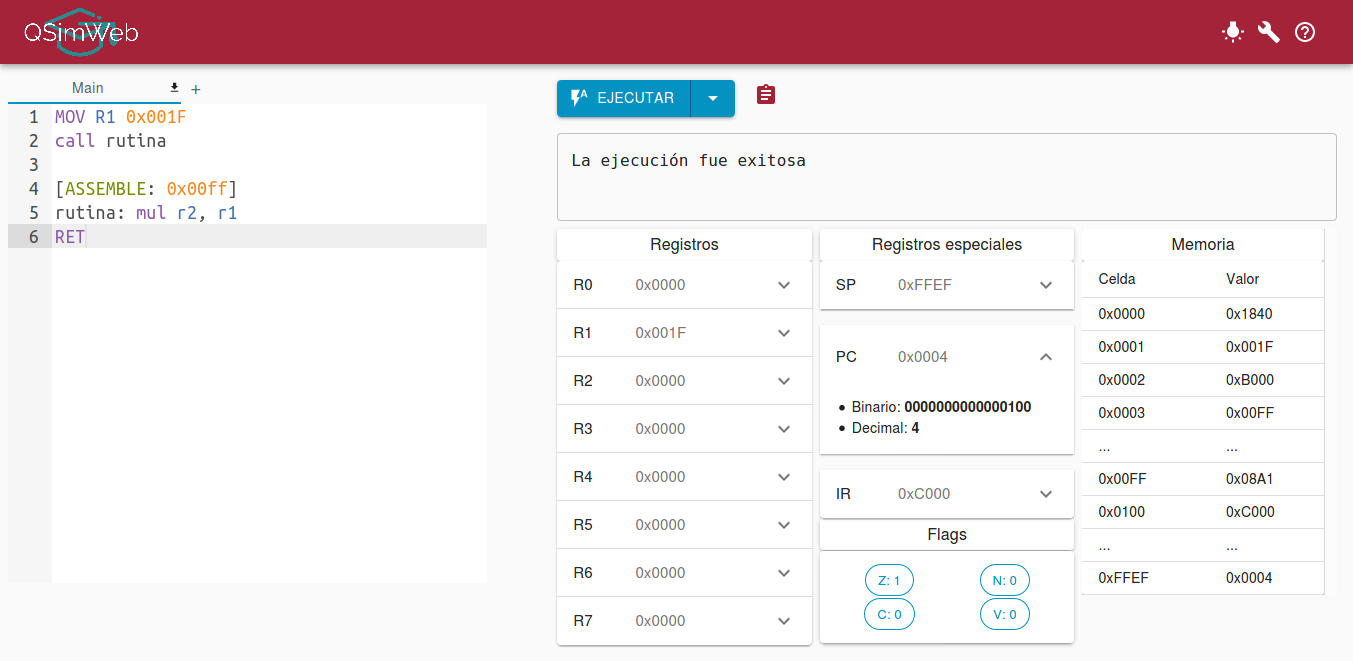
\includegraphics[width=14cm]{figuras/app-completa-bb.png}
\end{center}

\section{Proceso de ejecución}
Una de las necesidades principales es poder ejecutar código Q. La ejecución de un programa se compone de los siguientes pasos:

Se escribe un código Q en el editor de texto y se presiona ejecutar. 
Luego se analiza sintacticamente el texto que representa al programa, esta tarea es realizada por el Parser. 
Si ocurre un error se mostrará en pantalla informando lo ocurrido. Si el parseo pudo realizarse correctamente, se procede a 
traducir el resultado del parseo a instrucciones de la librería, esta tarea es realizada por el Translator.
Luego se procede a ensamblar y ejecutar el programa, ambas tareas son realizadas por Computer.
Si ocurre un error se mostrará en pantalla informando lo ocurrido. 
Si el programa finaliza, se mostrarán los resultados en pantalla.
\begin{figure}[H]
  \centering
  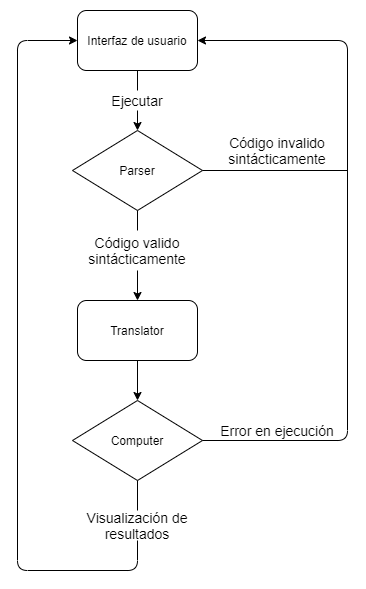
\includegraphics[width=10cm]{figuras/ejecucion_diagrama.png}
  \caption{Proceso de ejecución separado por componentes}
\end{figure}

Los detalles relacionados con la interfaz de usuario serán explicados en la sección que sigue a continuación.

Los detalles relacionados con la librería serán explicados en la sección ~\ref{qlib}


\section{Interfaz de usuario}

La interfaz cuenta con una pantalla inicial donde se pueden escribir y ejecutar programas Q, permitiendo visualizar los resultados de la ejecución. 
Además cuenta con una sección que permite configurar algunos aspectos de uso de la misma.

Se encarga de coordinar los pasos requeridos para ejecutar un programa utilizando la librería, es decir, parseo, traducción, ensamblado y ejecución del código. 

Las secciones nombradas anteriormente se describen a continuación:

\begin{center}
  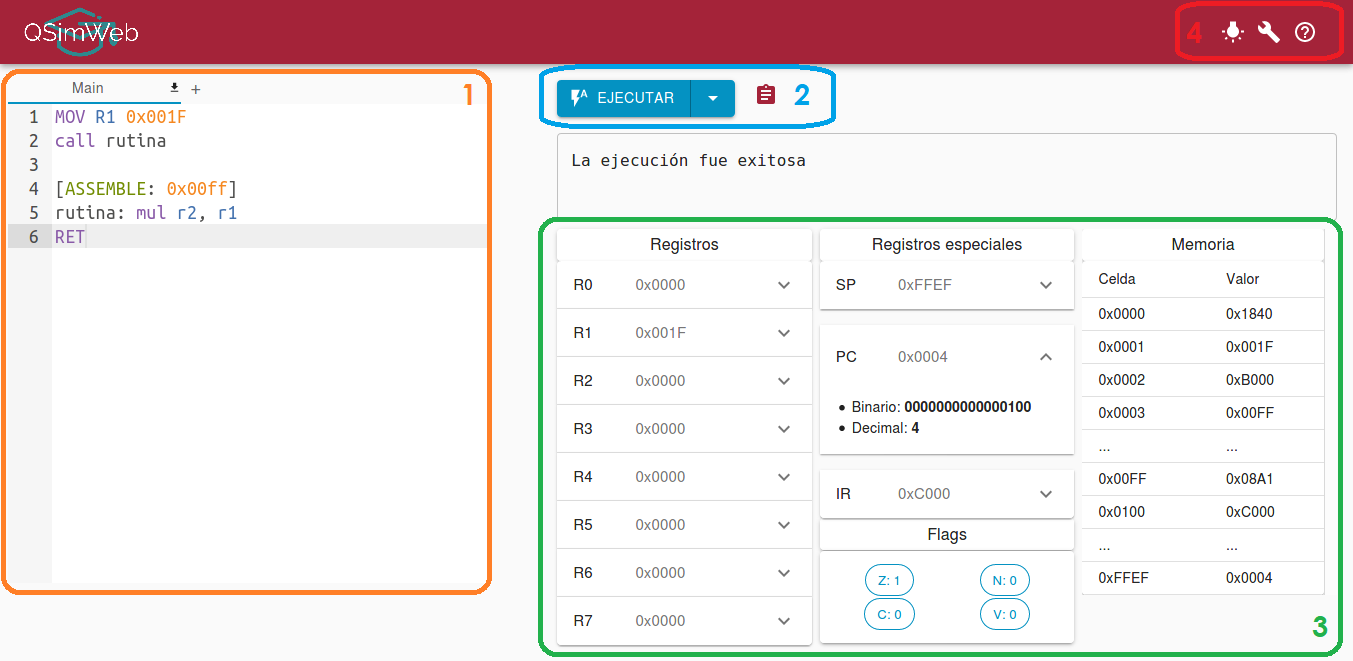
\includegraphics[width=14cm]{figuras/app-completa-dividida.png}
\end{center}

\subsection*{1. Editor}
Los programas se escriben sobre un editor de texto que cuenta con resaltado de sintaxis y errores. Estos programas pueden ser escritos tanto
en mayúsculas como en minúsculas. Cuando las instrucciones tienen más de un operando, estos pueden ser separados mediante uno o mas espacios o una coma.
El editor fue desarrollado utilizando la librería react-ace.

\begin{figure}[H]
  \centering
  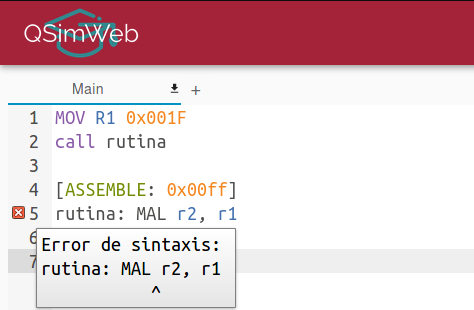
\includegraphics[width=10cm]{figuras/editor_errores.png}
  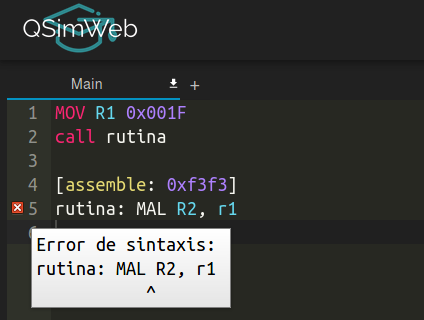
\includegraphics[width=10cm]{figuras/editor_errores_obscuro.png}
  \caption{Editor de texto con resaltado de sintaxis.}
  \label{fig:editor}
\end{figure}

Se permiten crear rutinas, ensamblandolas en celdas específicas utilizando [assemble: X], donde X es un inmediato representando la celda de memoria donde se ensamblará la rutina.
\begin{figure}[H]
  \centering
  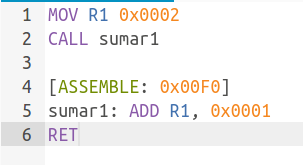
\includegraphics[scale=0.6]{./figuras/ASSEMBLE.png}
  \caption*{La meta instrucción ASSEMBLE permite indicar que la rutina sumar1 se ensamblará a partir de 0x00F0.}
  \label{fig:ASSEMBLE}
\end{figure}

\begin{figure}[H]
  La herramienta además permite la realización de comentarios que no afectarán la ejecución. Un comentario comienza con \# y termina al final de la línea.
  \begin{center}
    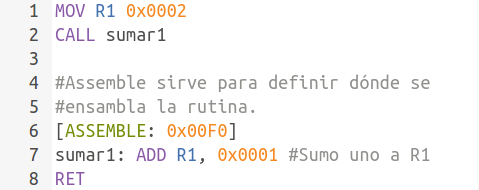
\includegraphics[scale=0.6]{./figuras/comentarios.png}
  \end{center}
  \label{fig:comentarios}
\end{figure}

\begin{samepage}
  Cuenta también con la posibilidad de dividir el código en distintas pestañas, importación de archivos .txt y descarga de los programas.
  
  \begin{center}
    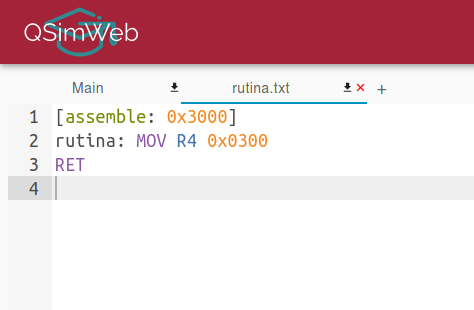
\includegraphics[width=10cm]{figuras/editor_tab.PNG}
  \end{center}
\end{samepage}

\subsection*{2. Botón de ejecución}
Cuando se quiere probar el código escrito, se debe ejecutar, haciendo click en el botón de ejecución.
La interfaz da la opción de ejecutar un programa de 3 modos distintos: Ejecución completa, Ejecución por instrucción y Ejecución por instrucción detallada. 
\begin{center}
  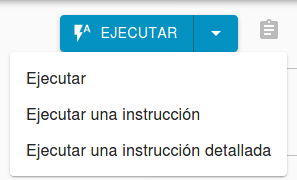
\includegraphics[width=7cm]{figuras/boton_ejecucion.png}
  \label{fig:boton-ejecucion}
\end{center}

El modo Ejecución completa realiza la ejecución de la totalidad de las instrucciones del programa mostrando, al final, los cambios en la sección de resultados. 

Ejecución por instrucción realiza la ejecución de una instrucción y muestra los cambios en la sección de resultados, al hacer click nuevamente, ejecutará la siguiente instrucción si existe. Si no existe se comenzará a ejecutar el programa nuevamente.

Para el modo de Ejecución por instrucción detallada, mostrará mensajes con las acciones producidas en cada paso de la ejecución. 

\begin{center}
  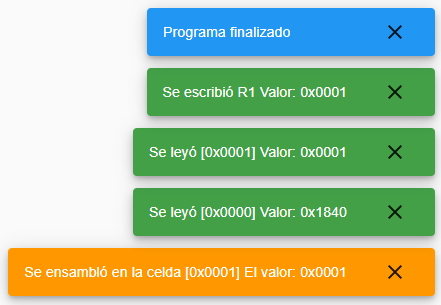
\includegraphics[width=8cm]{figuras/ejecucion_detallada.png}
\end{center}

En todos los modos de ejecución, dichas acciones quedan registradas y disponibles para su revisión:

\begin{center}
  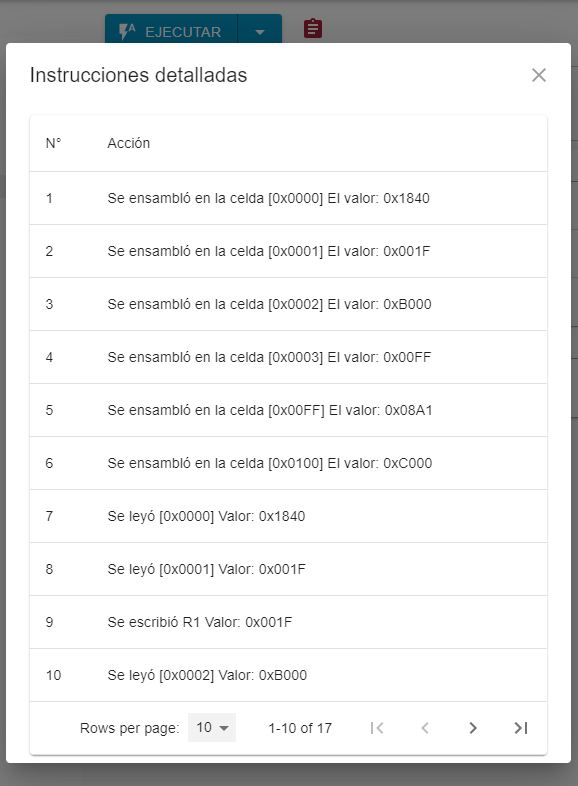
\includegraphics[width=9cm]{figuras/instrucciones_detalladas.PNG}
\end{center}

\subsection*{3. Resultados}
Una vez finalizada la ejecucion, con o sin errores, se actualizará la sección de resultados.

Los resultados se componen de los valores de registros, registros especiales, flags y memoria. Los valores de registros y registros especiales pueden ser
visualizados en hexadecimal, binario y decimal.
\begin{figure}[H]
  \centering
  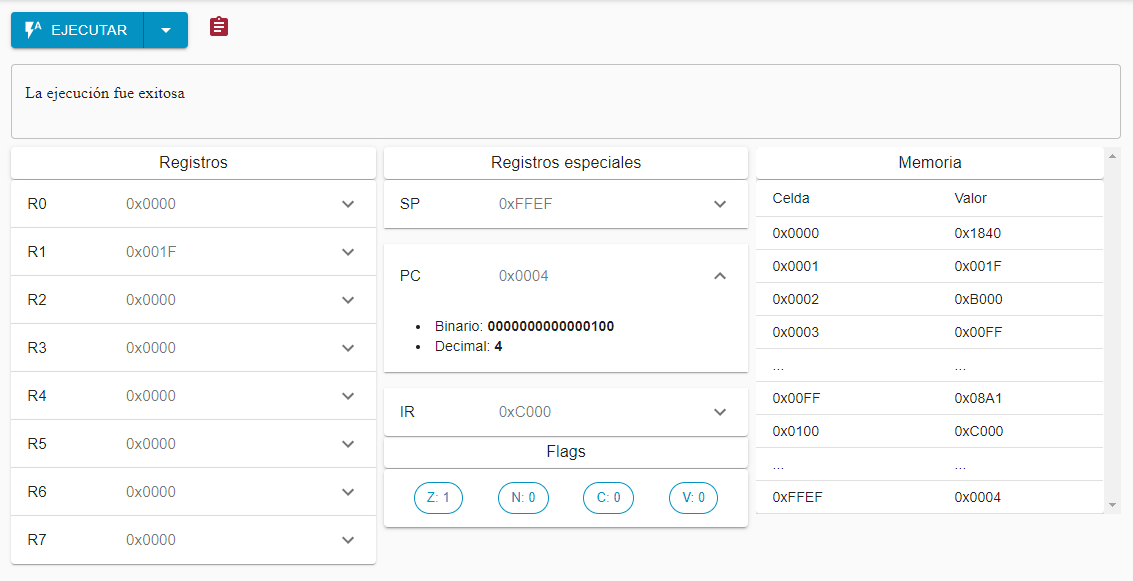
\includegraphics[width=14cm]{figuras/resultados.PNG}
  \caption{Resultados de la ejecución, separados en registros, registros especiales y memoria.}
  \label{fig:resultados}
\end{figure}

\begin{figure}[H]
  Cuando la memoria contiene celdas inicializadas que no son contiguas se resumen las celdas intermedias colocando "...".
  \begin{center}
    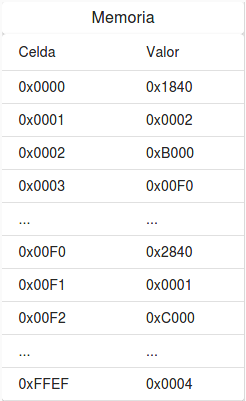
\includegraphics[scale=0.6]{./figuras/memoria_assemble.png}
  \end{center}
  \label{fig:memoria_assemble}
\end{figure}

Si durante la ejecución se produjo un error, este será mostrado en pantalla.
\begin{figure}[H]
  \centering
  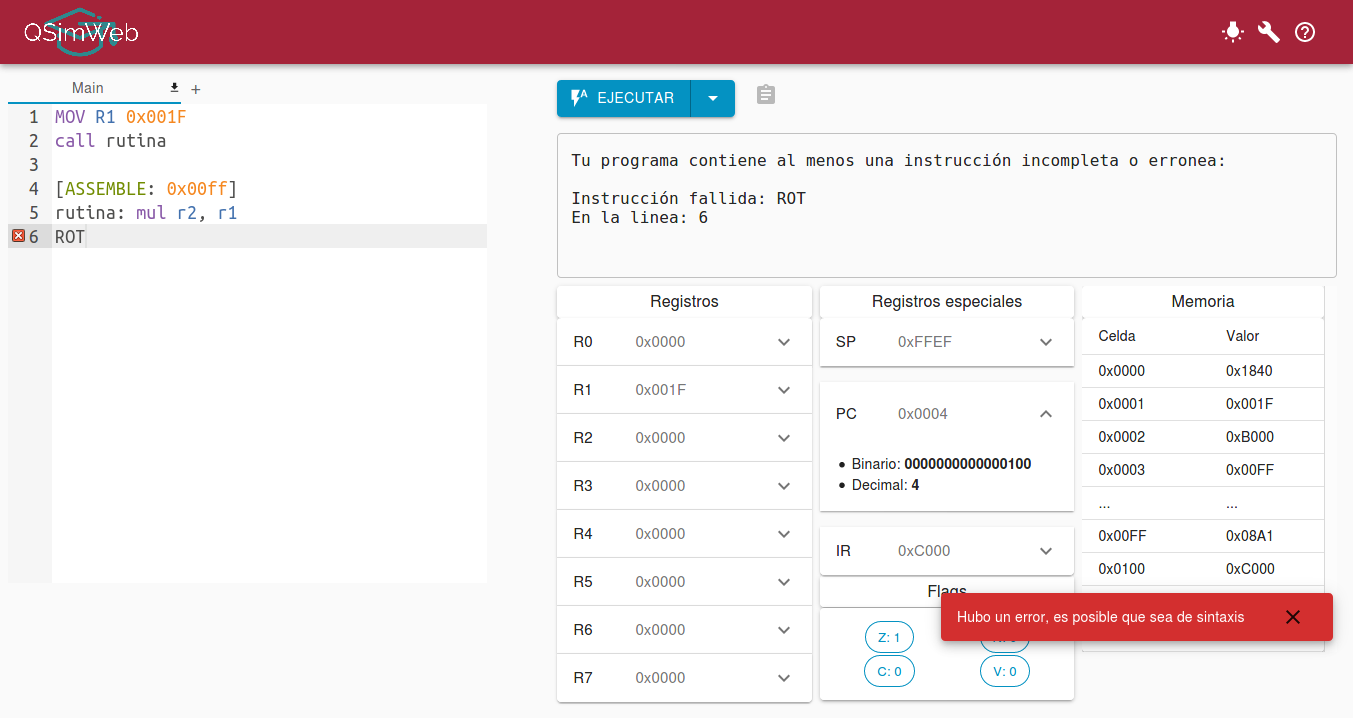
\includegraphics[width=14cm]{figuras/error.png}
  \caption{Error de sintaxis ocurrido al presionar ejecutar.}
  \label{fig:error}
\end{figure}

\subsection*{4. Configuraciones y ayuda}
La ventana principal cuenta además con un menú que permite configurar parametros de la ejecución.

\begin{center}
  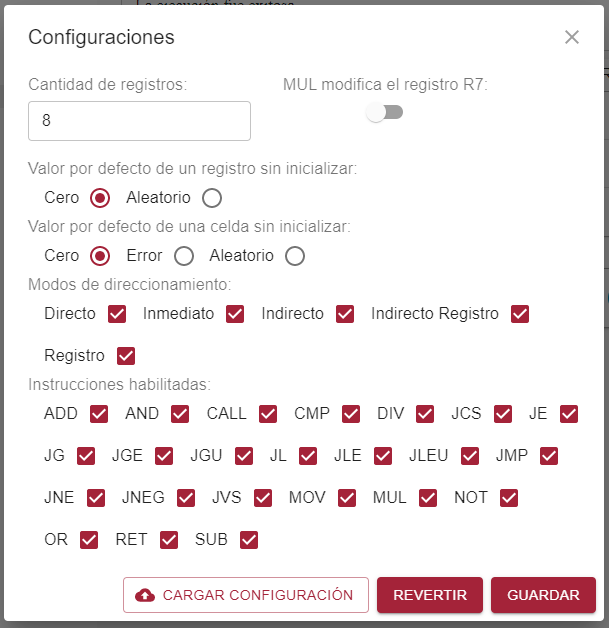
\includegraphics[width=8.7cm]{figuras/configuraciones.PNG}
\end{center}
En la configuración se permite cambiar la cantidad de registros, el comportamiento de MUL respecto al registro R7, los valores por defecto de las celdas de
memoria y registros, los modos de direccionamiento e instrucciones habilitadas. Es decir, todas las configuraciones que se especificarán en QConfig \referencia{subsec:qconfig}.
Además permite cargar un archivo de configuración para simplificar el armado de la misma.

Estas prefencias mencionadas se guardan en el navegador del usuario, permitiendo que no se pierdan al finalizar su uso.
Además se permite importar un archivo de configuración, donde se pueden especificar las configuraciones nombradas anteriormente. 

Se permite además ver un manual de uso.
\begin{center}
  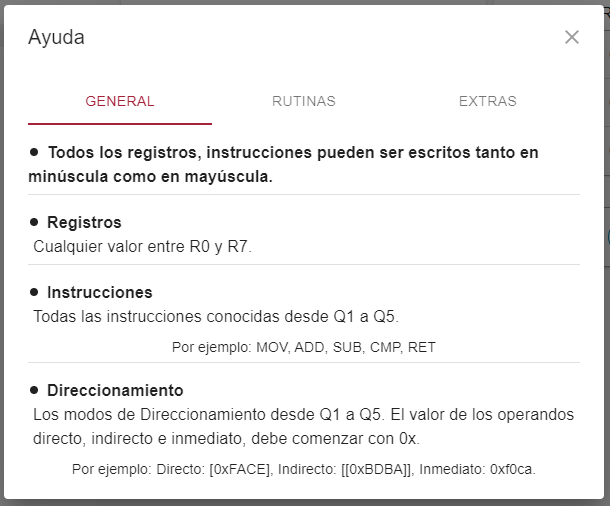
\includegraphics[width=8.7cm]{figuras/ayuda_general.PNG}
\end{center}

Existen los modos oscuro y claro, que facilitan el uso por parte de personas con daltonismo.
\begin{center}
  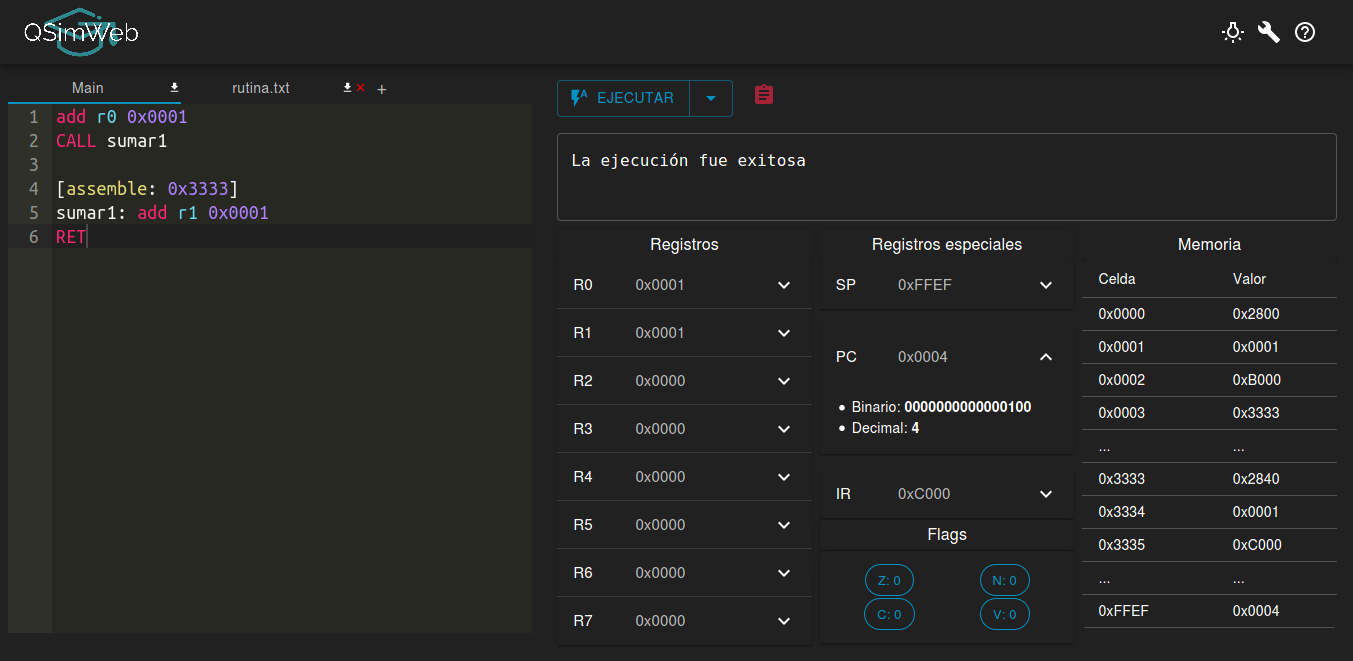
\includegraphics[width=14cm]{figuras/modo_obscuro.png}
\end{center}
\end{itemize}

\subsection{Accesibilidad}
\label{accesibilidad}

Una de las funcionalidades esperadas era brindar la posibilidad de la herramienta de ser usada con lectores de pantalla. En este sentido
se hicieron evaluaciones de accesibilidad utilizando herramientas estandarizadas y una prueba de campo con un estudiante no vidente de la tecnicatura.
Dichas evaluaciones permitieron hacer un diagnóstico de accesibilidad y posterior corrección de las fallas encontradas. Actualmente la 
herramienta contiene código para facilitar su uso, permitiendo que se pueda acceder a todas las funcionalidades de la misma.

Las mejoras realizadas hasta el momento fueron:
\begin{itemize}
  \item Nombrar correctamente el lenguaje de la aplicación ya que react pone por defecto el lenguaje en inglés.
  \item Agregar etiquetas a todos los botones.
  \item Agregar encabezados a la sección de resultados, para permitir su navegación y lectura.
  \item Corrección de autofoco en los modales.
  \item El contenido de las ventanas emergentes se lee automáticamente por el lector de pantalla.
\end{itemize}
